\documentclass[11pt]{article}
\usepackage[margin=1in]{geometry}
\usepackage{graphicx,booktabs,amsmath,amssymb,hyperref}
\hypersetup{colorlinks=true,urlcolor=blue,citecolor=blue,linkcolor=blue}
\setlength{\parindent}{0pt}
\setlength{\parskip}{0.35em}
\setlength{\emergencystretch}{2em}
\title{Early Answers, Late Exits:\\Availability and Execution Costs in Frozen NCM}
\author{Anytime NCM project\\{\small Internal review draft: human authors and affiliations unconfirmed}}
\date{24 October 2026 --- version 4}
\begin{document}
\maketitle
\begin{abstract}
Useful adaptive generation needs acceptable early outputs, a causal recognition signal, and enough saved execution to cover observation costs. We examine these requirements in released frozen Next-Concept Modeling checkpoints. Historical Sudoku audits found no early exact valid solutions; a bounded saved-WMT assignment search found point-feasible outputs but failed conditional quality bounds. We then prospectively audited 256 separately assigned WMT14 groups and measured all fixed depths and a clairvoyant exact-final-text assignment. Early text identical to the same input's full output occurs on 43/256 inputs, mostly near the final level. With every-level observation charged, the assignment averages 146.56 ms versus 129.23 ms at full depth, 13.41\% overhead with adjusted reduction interval [-15.21\%,-11.31\%]. All fixed early depths fail an adjusted corpus-quality endpoint. A subsequent explicitly post hoc screen assembles the same exits from existing terminal-only measurements: even omitting earlier inspections, estimated savings are only 2.67\%, exploratory interval [1.74\%,3.73\%], below the 5\% target. The latter is not a new online-policy benchmark or a global bound. These bounded results distinguish early-answer presence from sufficient economic headroom; they do not prove universal failure of adaptive NCM, a causal mechanism, or absence of useful approximate outputs. Controller and final-confirmation branches remain unexecuted.
\end{abstract}

\section{Question and contribution}
NCM generates a hierarchy of discrete codes and reconstructs outputs from cumulative representations~\cite{ncm}. We ask whether released, frozen checkpoints can stop at different levels per input while retaining acceptable quality and improving actual ready-output latency over full depth and a strong fixed-depth control.

The contribution is a controlled negative diagnostic separating three requirements: \emph{availability}, \emph{causal recognition}, and \emph{execution economics}. Presence of a satisfactory prefix does not establish an affordable decision rule. Conversely, failure of selected policies does not prove satisfactory prefixes absent. We report which observations resolve these distinctions and which remain unknown, without proposing a new stopping algorithm or claiming novelty priority.

This version includes the completed E0--E2 extension and a post hoc terminal-cost screen. Version 3, its compiled PDF, original protocols, sources, failures and receipts remain unchanged. This is an internal local review draft, not a submission-ready or peer-reviewed paper. A project label is not a verified human byline.

\section{Relation to adaptive inference}
NCM uses nested dropout to encourage informative partial reconstructions; informative prefixes do not guarantee exact task acceptance or inexpensive observation~\cite{ncm}. Depth-Adaptive Transformer trains intermediate decoder predictions~\cite{dat}. CALM addresses confidence and sequence-level consistency in adaptive autoregressive decoding~\cite{calm}; calibrated risk control requires its own assumptions and procedure~\cite{ltt}. These approaches adapt Transformer layers, whereas our frozen NCM studies stop code levels before a separate reconstruction and decoder path. Their guarantees and speedups are not transferred numerically to this setting.

ACT and PonderNet learn computational allocation during training~\cite{act,ponder}. Optimal stopping distinguishes a realizable rule from an optimal-value certificate~\cite{optimal}; stopping across additional candidate generations is another setting~\cite{bestn}. We trained no true continuation-value estimator. Current answer validity, eventual failure, and expected incremental utility are different targets. Any future causal model would have to use only its actual current/past observation history and account for the cost of obtaining that history.

Corpus resampling in MT motivates paired analysis~\cite{koehn}, but it does not solve outcome-dependent search, unknown document dependence or rare-cue coverage. The repository includes a broader, explicitly bounded primary-source reading note. This manuscript is not a systematic review.

\section{Historical evidence and remaining uncertainty}
Historical hard and extended easy Sudoku audits each inspected 1,400 exploration/development trajectories and found no early exact valid board in their respective settings. A 32-target encoding pilot had exact final round trips but no early valid target reconstruction. This narrows a question; it does not identify a generator-only or decoder-only cause. Related Sudoku studies share source solutions and are not independent populations to pool.

Selected historical verified/learned Sudoku and WMT policies reached full depth and added overhead. The learned Sudoku controller estimated current validity, not continuation value. The WMT policies' final-only behavior concerns those policies, not every possible exit. A viewer and saved Concept Firewall forecast bridge are inspection tools, not additional evidence of speedup, efficacy or safety.

The stronger saved-WMT study used 128 reused exploration and 64 reused development groups. Six deterministic coordinate searches exhausted 60,000 charged assignments. A development assignment exited early on 18/64 inputs, with point losses 0.370429 BLEU and 0.984773 chrF inside the 0.5/1.0 margins. A dimensionless monitored-cost surrogate estimated 9.016\% savings, conditional interval [2.799\%,15.778\%]. Conditional one-sided quality lower bounds, -1.163781 BLEU and -1.905485 chrF, failed noninferiority. Those optimized assignments were not timed at arbitrary exits. A best feasible assignment found is not a certified optimum; keeping selected assignments fixed in bootstrap also ignores search-selection uncertainty.

The saved diagnosis found visible early/final equality on 17/128 exploration and 13/64 development inputs, versus raw 64-ID equality on 2/128 and 1/64. Rendering can hide token differences. These are descriptive observations, not semantic correctness, a usable online signal or a demonstrated mechanism. Earlier savings estimates remain estimates; the later measured E2 assignment is a different rule/population and does not retrospectively calibrate S1.

\section{Prospective E0--E2 design}
\subsection{Population, exposure and release}
The released WMT pool has 3,003 distinct effective 96-token source-prefix groups. An input-only audit also checked exact source duplication and recorded-access paths. It did not recover document identities or establish checkpoint-training independence. Among 1,979 historical reserved groups, E0 fixed 256 for E2 audit, 128 for conditional development, 1,024 for conditional confirmation and 571 closed/unallocated. Allocation sorts SHA256 of a fixed salt plus identity, with canonical index ties. Those groups already had official aggregate-baseline exposure; E0 later hashed source strings. They were not untouched examples.

E2 separately released only its 256 groups after protocol/source push, remote equality and asset preflight. The E0 allocation remains immutable; a new release receipt records the access transition. E2 is consumed diagnostic/development evidence, not fresh policy confirmation. E3/E4 and the unallocated groups remain closed. Warmups use only 16 previously exposed exploration identities. No new confirmation outcome is inspected.

Pinned released code, checkpoint, data and text-tokenizer revisions are in Appendix~\ref{app:repro}. A nonexecuting selective string reader restricts source/reference materialization. No Qwen language-model weights are used. WMT has 11 levels of widths
\[
(1,4,8,14,20,26,32,40,48,56,64),
\]
313 total codes and 64 decoded target IDs. Every prefix uses the released learned full-resolution reconstruction cascade; independent snapshots, suffix isolation and all-level parity have separate implementation checks.

\subsection{Statistical feasibility and prospective narrowing}
Quality tolerances remain corpus BLEU loss 0.5, chrF loss 1.0, numeric-reference F1 loss 0.02 where defined, and negation-mismatch increase 0.02. Corpus SacreBLEU 2.6.0 sufficient-statistic sums match direct corpus scoring. Literal number/negation cues are heuristics, not factuality or safety guarantees.

E0's input-only/synthetic preflight found the proposed nonidentical-output E2 gate infeasible at \(n=256\) under its conservative signed rare-cue envelope. For paired differences in [-1,1], the envelope is
\[
[-U(n_-,n,\alpha),\,U(n_+,n,\alpha)],
\]
where \(U\) is a one-sided Clopper--Pearson upper binomial probability and \(n_-,n_+\) count negative/positive differences. It discards favorable offsets and magnitudes deliberately. With zero adverse events its upper bound is \(1-\alpha^{1/n}\), not zero.

The original 89-interval design needed 405 covered examples at the 0.02 margin. E2 therefore dropped two nonidentical-output rules \emph{before outcomes}, keeping one exact-text rule and all 11 fixed controls. Its 59-interval family still needs 385 covered examples for a nonidentical rule. Actual E2 numeric coverage is 48/256. Inadequate coverage cannot silently count as noninferiority; the exact rule has a different structural equality property. Changing a statistical method after these outcomes could not retroactively rescue the gate.

\subsection{Exact assignment, controls and actual clocks}
Collect one full 11-prefix trajectory per E2 input. Choose the earliest level whose rendered Python string exactly equals that input's level 11 string, otherwise 11. No normalization, reference-based threshold, assignment optimization or subset selection is allowed. This clairvoyant assignment is a diagnostic label, never an online feature.

Measure 12 methods: the assignment with every-level observation to its forced exit, and terminal-only fixed depths 1--11. Terminal 11 uses unchanged native full generation/reconstruction. Other terminal depths use a validated hard maximum and one decode; every-level execution reconstructs/decodes all visited levels. Precomputed exit selection is outside the request clock, while all charged observation work is inside. This measures execution of assigned exits, not causal recognition or end-to-end oracle search.

Use one collection process and two separately started timing processes, two paired repeats per method/input/process, plus five warmups per method/process. Method ordering and reversed input ordering are frozen. The allocation is 256 collection +12,288 timed +120 warmup =12,664 requests. Upper generator/decoder work is 82,434/25,564 sample forwards; actual work is 82,110/25,240. Encoder forwards, target encodings, fits and weight updates are zero. All requests, including warmups, count; no retries or replacements occurred.

On the existing RTX 5060/WSL2 environment, models run float32/eval, batch one, four CPU threads, with no autocast or compilation. Torch 2.10.0+cu 128, CUDA 12.8 and Transformers 4.57.6 are recorded. Source preprocessing, transfer, reconstruction, decoding and CPU text readiness enter synchronized wall latency. Loading, state hashing, parity serialization and offline reference analysis are recorded separately. CUDA-event stream span is secondary and not kernel busy time. Every scheduled code prefix, observed ID sequence and text matches its collected output; every model-state fingerprint is unchanged. This includes native-full versus collected-hook parity without extra requests.

\subsection{Uncertainty and practical gate}
Average repeats within identity/process, then weight identities and process blocks equally. Exactly 100,000 shared identity vectors and crossed process vectors, seed 20261026, retain all methods together. Corpus metric differences sum resampled statistics; cue intervals use the signed envelope above. The simultaneous family has 48 quality intervals and 11 exact-versus-fixed cost intervals, tail \(\alpha=0.05/(2\cdot 59)\), including structural/full-self redundancies without alpha reuse.

An additional 0.001 Monte Carlo rank allowance gives one-based rank 18 for guarded bootstrap tails; unresolved ranks cannot pass. This numerical allowance is not a sampling-model guarantee. Two process sessions and unknown document dependence limit generalization. Structural exact-text equality makes relative deterministic text quality exactly zero, conditional on parity; a fixed early method that only happens to match finite observed outputs does not inherit that guarantee.

Require at least 5\% point mean reduction versus full with positive adjusted lower bound, plus positive adjusted lower savings versus every potentially feasible fixed depth. Exclude a fixed depth only when an adjusted quality interval lies wholly beyond a margin. Otherwise retain it, including uncertain or sparse-cue cases. A full-relative upper savings bound below 5\% is a bounded no-go. No rule/schedule enlargement follows a negative gate.

\section{Prospective results}
E1, a cost pilot on 16 reused inputs, completed 1,000 allocated requests with matched cached parity. Terminal depth 10 averaged 117.52 ms versus 127.36 ms full, while every-level observation through 10 averaged 135.76 ms. Those are engineering measurements without quality evaluation; they justified considering E2, not a matched-quality speedup.

\begin{table}[ht]
\centering\small
\begin{tabular}{lrrrr}
\toprule
E2 method & Mean ms & p 95 ms & BLEU & chrF\\
\midrule
Every-level exact assignment &146.557&158.928&23.018&50.903\\
Terminal fixed 10 &118.469&125.582&19.277&47.013\\
Native terminal 11 &129.230&137.266&23.018&50.903\\
\bottomrule
\end{tabular}
\caption{Same 256 E2 audit inputs. These are actual request costs; only the assignment is clairvoyant. Fixed 10 is faster but fails quality. Full-relative exact quality equality is structural, not semantic correctness. All 12 methods are retained in the machine-readable record.}
\label{tab:e 2}
\end{table}

The earliest exact match occurs on 43/256 inputs (16.797\%): level 6: 1 input; level 7: 3; level 8: 6; level 9: 13; level 10: 20. The remaining 213 require level 11. None of levels 1--5 matches the final rendered string in this audit. Mean assigned depth is 10.683594. Work counts are not latency savings.

The exact assignment is \textbf{13.407\% slower} than full. Its adjusted relative reduction interval is[-15.208\%,-11.310\%], wholly below the+5\% target. Process-specific reductions are-13.443\% and-13.372\%. Thus the practical gate fails even before causal recognition is attempted. All fixed depths 1--10 fail at least one adjusted corpus-quality endpoint; only full depth remains potentially feasible. Fixed 10 loses 3.7411 BLEU, interval [-5.3757,-2.2709], and 3.8906 chrF, interval [-5.0439,-2.7786]. Neither passes the 0.5/1.0 contract.

\begin{figure}[ht]
\centering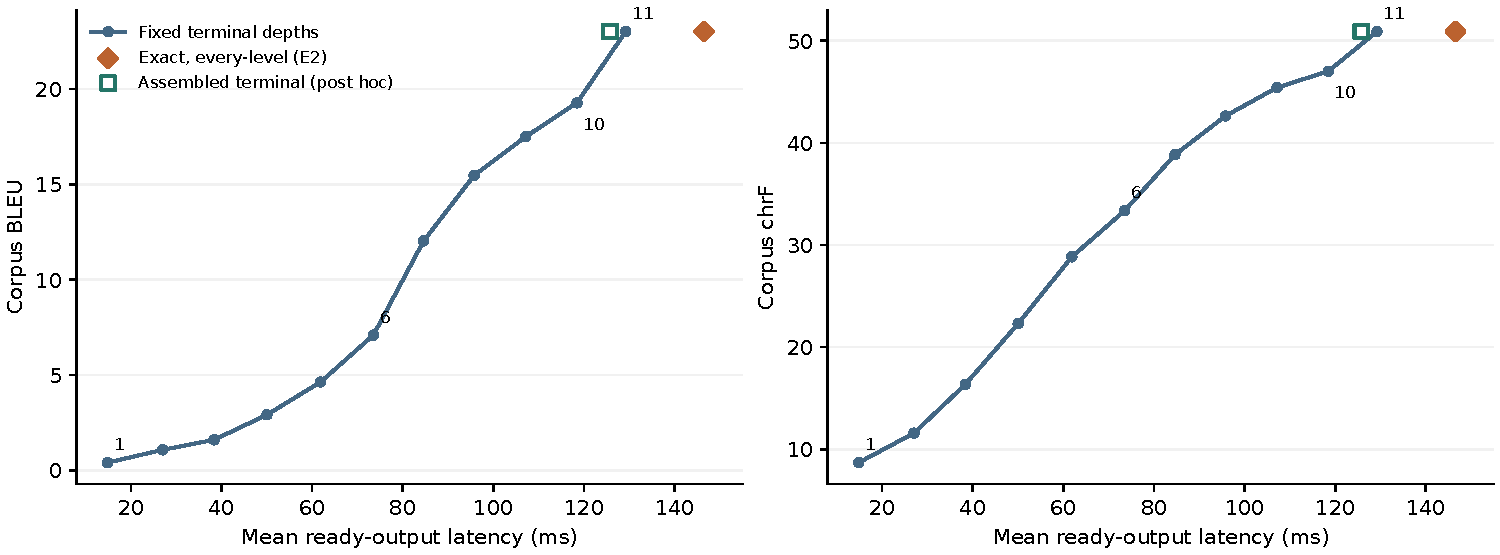
\includegraphics[width=\linewidth]{figures/quality-latency.pdf}
\caption{E2 corpus-quality points and measured mean request costs. Connected points are fixed terminal depths, not a certified optimal frontier. Exact every-level execution preserves full text but costs more. The square is the separately labeled post hoc assembled terminal screen in Section~\ref{sec:screen}, not a measured causal policy. Points omit quality intervals for legibility; the gate uses the recorded adjusted bounds.}
\label{fig:latency}
\end{figure}

\begin{figure}[ht]
\centering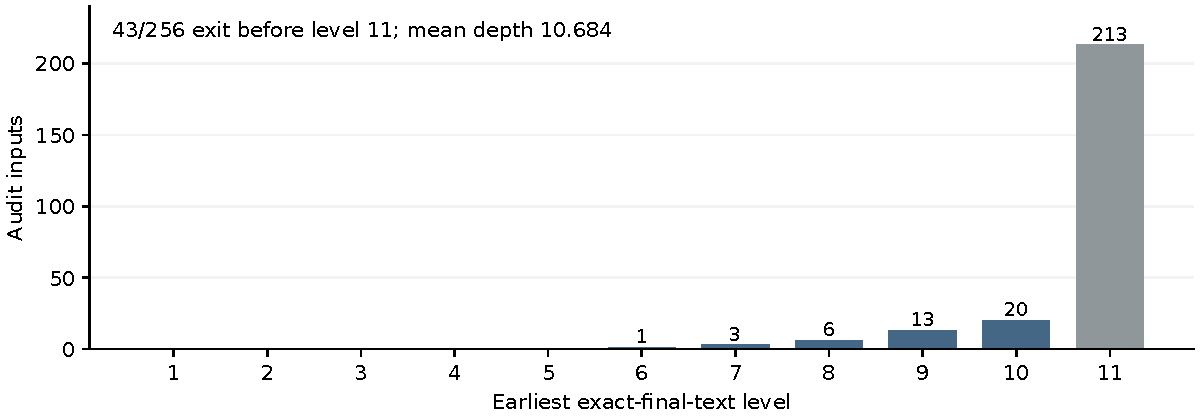
\includegraphics[width=.84\linewidth]{figures/exact-depths.pdf}
\caption{Earliest exact-final-text level in the preassigned 256-group audit. Exact early outputs exist but are sparse and late. This does not characterize all semantically useful approximate outputs or identify a cause in the model.}
\end{figure}

\section{Post hoc terminal-cost screen}\label{sec:screen}
E2 left open whether every-level observation alone hid a worthwhile earliest-exact opportunity. After seeing E2 and fixed-method aggregates, we froze a saved-data-only screen before calculating its selected-terminal aggregate. This choice is \emph{post hoc}, not prospective confirmation.

For each E2 identity/process/repeat, select the already measured fixed-terminal request at its earliest exact level. Average these cells and compare with paired full and dense-exact cells. Earlier inspections and decision computation are deliberately omitted. Constituent request latencies are measurements, but the assembled result is neither an integrated selector benchmark nor a bound on every possible exact assignment/schedule. Earliest depth does not certify minimal real latency.

Selected terminal cells average 125.779 ms versus 129.230 full: \textbf{2.670\% savings}, exploratory interval [1.735\%,3.729\%]. The two process points are 2.666\% and 2.674\%. Even this deliberately optimistic construction falls below 5\%. Every-level exact cells cost 16.519\% more than assembled terminal cells, interval [16.051\%,16.970\%]; the difference includes schedule/implementation-path effects and is not a pure decoder-cost decomposition.

The screen reuses E2's 100,000 identity/process vectors, with a local two-contrast tail 0.0125 and numerical rank 1130. These exploratory intervals are not joint confirmatory guarantees across the research sequence or a correction for choosing this question after E2. No reference read, new model call, candidate search or fit occurs. A separate arithmetic check reproduces all 3,072 selected values and both intervals. The operational decision is not to budget more inference for this same earliest-exact rule, not to declare a global impossibility result.

\section{Interpretation, gaps and stopping}
The data distinguish a complete absence of early full-answer text from insufficient economic headroom for the tested rule. In WMT, some such text exists. With the prospective dense schedule, saved refinement fails to offset observation work. The post hoc screen further suggests that eliminating earlier inspections alone would not meet the chosen target for these earliest-exact assignments. The latter is a budget-priority observation on consumed data, not a new gate pass or causal proof.

We have not established useful tolerated nonidentical-output opportunities under adequate rare-cue bounds, a cheaper successful sparse schedule, a recognizable continuation-value signal, an optimal assignment, or the origin of intermediate-code errors. Target encoding would not uniquely isolate an actionable intervention from this evidence. The same-assistant calculations do not replace independent scientific review, and the statistical assumptions need critical review.

Controller development (S3/E3) remains blocked; E4 confirmation stays closed. Target encoding/intervention (S2B/M1/S4) is deferred rather than implemented. An alternative scientific direction needs a specific contrast, prospectively defined eligibility/statistics/resources and honest reuse of E2 as development evidence. No samples, margins or candidate families are enlarged simply to find a positive result.

The local hard-Sudoku official aggregate is 1,725/2,000=86.25\%, versus the publication's 86.1\%. A bounded metadata review rejects rounding alone as an explanation but cannot identify a cause. Published general runtime specifications and local release receipts are not matched execution evidence. The discrepancy remains unexplained; no rerun or score correction was performed.

The defensible outcome is a bounded negative study of availability and execution costs. It supports neither universal failure of adaptive NCM nor factuality/safety guarantees. Human authors must assess the contribution, verify responsibility/rights and arrange independent review before any publication decision.

\appendix
\section{Provenance, access and reproduction}\label{app:repro}
\begin{center}\footnotesize
\begin{tabular}{lp{.64\linewidth}}
\toprule
Source & Recorded revision\\
\midrule
NCM code & \texttt{c70274273f489abc73832b2b98584a8483b6b203}\\
Checkpoint & \texttt{d342ce8aaea58830eef3b8ad473664673e41f692}\\
Dataset & \texttt{6580ba41a4b0a976dde876fbe84d25327617b0e6}\\
Text tokenizer only & \texttt{c1899de289a04d12100db370d81485cdf75e47ca}\\
\bottomrule
\end{tabular}
\end{center}
{\raggedright At manuscript preparation the evidence baseline is repository \texttt{298f2e6}. E2 source was frozen/pushed at \texttt{d88b7c4}; completed records at \texttt{d84b2a4}. The screen source was pushed at \texttt{598364c} and closure at \texttt{7db4d08}. M0's locked archival review closes with cause unresolved. Full digests and exact executed working-tree bytes are in source archives; Git LF normalization need not preserve Windows CRLF bytes.\par}

The accompanying review packet maps claims to protocols, aggregate records and limitations. It includes the E0 role manifest, separate E2 access release, failure/attempt pointers, code/asset digests, review questions and human-action list. Data/weights are not bundled; their required local assets and unresolved access/rights are stated. Source archives can support reproduction in a separate checkout, never silent replay of consumed allocations.

Historical full-suite evidence is 451 passing tests at its recorded snapshot. E2 ran 96 focused synthetic/compatibility tests before its model execution. The terminal screen ran 32 focused synthetic tests. These counts are not additive independent experiments or a fresh whole-suite claim. Separate checkers reproduced E2 ledgers/direct corpus points/cue envelopes/timing intervals and terminal-screen arithmetic; corpus bootstrap was not independently reimplemented by another scientist. No final-policy verifier is rerun merely to refresh this manuscript.

\section{Work, clocks and resource accounting}
E1 completes 1,000 requests/6,600 generator evaluations/3,800 decoder forwards on exposed inputs. E2 completes 12,664/82,110/25,240, including collection and warmups, with no failures/retries. E2 model orchestration takes 1,129.041 seconds, analysis 32.116 seconds, with a conservative 10,800-second preparation/report charge. Its analysis peak RSS is 758,616,064 bytes and original execution artifacts 23,806,383 bytes. Model loads are separately recorded in three process receipts.

The terminal screen has zero model work, 2.115 seconds recorded calculation, peak RSS 685,694,976 bytes and a conservative 6,300-second preparation/report charge. M0 charges its full two-hour archival allowance. P1 local synthesis is capped at four CPU hours/256MiB, with no new outcomes or model work. Allocated ceilings and conservative charges are not measured inference latency. All paid compute charges are zero; no dependency download, fit or training is used.

The 512 E2 reference materializations are two permitted reads of the same 256 references (execution and verification), not 512 independent quality inputs. Timing repeats and different precision/session observations cannot create new source-group samples. Known group separation does not establish document or checkpoint-training independence. Confirmation remains reserved and unobserved.

\section{Disclosure and remaining human decisions}
Substantial AI assistance contributed to code, analysis, literature synthesis and writing. Verified human author names, affiliations, scientific responsibility, project/data/model rights and license decisions are not supplied by repository ownership. The packet is for local review only. Independent researcher review, any reviewer contact, upload, endorsement/account checks and submission have not occurred. No person was contacted. No venue acceptance, novelty priority or general scientific approval is claimed.

\begin{thebibliography}{9}
\footnotesize\raggedright
\bibitem{ncm} H. Kumbong et al. Next-Concept Modeling: Fast, Parallel Coarse-to-Fine Text Generation. 2026. \href{https://arxiv.org/abs/2610.14162v1}{arXiv:2610.14162v1}.
\bibitem{dat} M. Elbayad, J. Gu, E. Grave and M. Auli. Depth-Adaptive Transformer. ICLR,2020. \href{https://arxiv.org/abs/1910.10073v4}{arXiv:1910.10073v4}.
\bibitem{calm} T. Schuster et al. Confident Adaptive Language Modeling. NeurIPS,2022. \href{https://arxiv.org/abs/2207.07061v2}{arXiv:2207.07061v2}.
\bibitem{ltt} A. N. Angelopoulos et al. Learn then Test: Calibrating Predictive Algorithms to Achieve Risk Control. 2022 revision. \href{https://arxiv.org/abs/2110.01052v5}{arXiv:2110.01052v5}.
\bibitem{act} A. Graves. Adaptive Computation Time for Recurrent Neural Networks. 2017 revision. \href{https://arxiv.org/abs/1603.08983v6}{arXiv:1603.08983v6}.
\bibitem{ponder} A. Banino, J. Balaguer and C. Blundell. PonderNet: Learning to Ponder. 2021. \href{https://arxiv.org/abs/2107.05407v2}{arXiv:2107.05407v2}.
\bibitem{optimal} S. Becker, P. Cheridito and A. Jentzen. Deep Optimal Stopping. JMLR20(74),2019;2020 revision. \href{https://arxiv.org/abs/1804.05394v4}{arXiv:1804.05394v4}.
\bibitem{bestn} Y. Kalayci, V. Raman and S. Dughmi. Optimal Stopping vs Best-of-N for Inference Time Optimization. 2025. \href{https://arxiv.org/abs/2510.01394v1}{arXiv:2510.01394v1}.
\bibitem{koehn} P. Koehn. Statistical Significance Tests for Machine Translation Evaluation. EMNLP,2004. \href{https://aclanthology.org/W04-3250/}{ACL Anthology W04-3250}.
\end{thebibliography}
\end{document}
